\edef\mychapter{Inequalities}
\edef\mychapterdate{July 7, 2024}

\chapter{\mychapter}

\section{Basic Inequalities}
\subsection{Increasing or Decreasing}
In this section, we will introduce the notion of an increasing or decreasing function. Generally, this concept is pretty easy to visualize on a plot for example in figure \eqref{fig:inc}, we can observe an increasing function.
\begin{figure}[h]
\centering
	\begin{tikzpicture}
		\begin{axis}
			\addplot[blue, thick,domain=0:3]{exp(x)};
		\end{axis}
	\end{tikzpicture}
	\caption{Plot of $e^x$.}
	\label{fig:inc}
\end{figure}
Then in figure \eqref{fig:dec}, we can observe $-\ln(x)$ is an example of a decreasing function.
\begin{figure}[h]
\centering
	\begin{tikzpicture}
		\begin{axis}
			\addplot[blue, thick,domain=0.01:3, samples=100]{-ln(x)};
		\end{axis}
	\end{tikzpicture}
	\caption{Plot of $-\ln(x)$.}
	\label{fig:dec}
\end{figure}
However, these declarations are only applied to a specific subset of all possible functions.
\begin{figure}[h]
\centering
	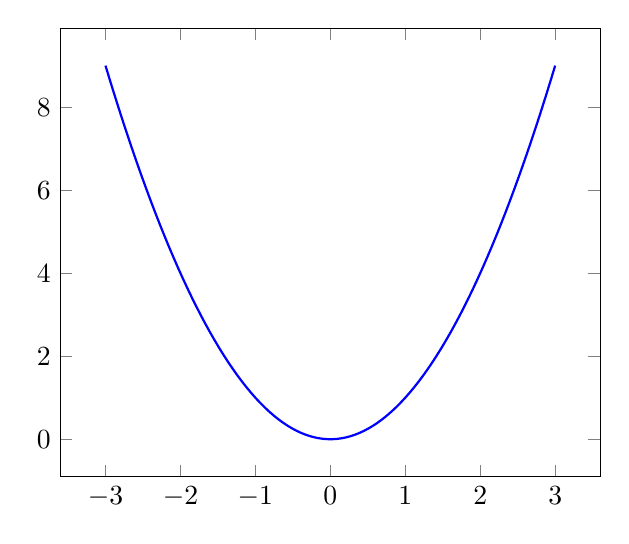
\begin{tikzpicture}
		\begin{axis}
			\addplot[blue, thick,domain=-3:3, samples=100]{x^2};
		\end{axis}
	\end{tikzpicture}
	\caption{Plot of $x^2$.}
	\label{fig:neith}
\end{figure}
In figure \eqref{fig:neith}, we can observe a function that is neither increasing nor decreasing. But it is here, that we note that whether a function is increasing or decreasing also heavily depends on what domain we define the function on. Had we restricted the domain to $x\ge0$ in figure \eqref{fig:neith}, we would get an increasing function.

Now with this basic intuition, let's define these ideas more rigorously with mathematics.

\begin{define}
Let $f:\real\to\real$\footnotemark be an increasing function. Then $a<b$ implies $f(a)\le f(b)$.
\label{def:inc}
\end{define}
\footnotetext{Technically, this is defined for any ordered set with a notion of "biggness", but for this introductory course, we will restrict ourselves just to $\real$.}
\begin{define}
Let $f:\real\to\real$ be a decreasing function. Then $a<b$ implies $f(a)\ge f(b)$.
\end{define}

Now had we exchanged the non-strict inequalities for strict equations, so $f(a)<f(b)$ and $f(a)>f(b)$ respectively, we would get the definition for a \textbf{strictly increasing} and \textbf{strictly decreasing} function. Now it must mentioned, that with the mathematical machinery that we have, it is rather difficult to prove any arbitrary real function is increasing or decreasing, so we will pick this up in a later lesson.

\subsection{Solving Basic Inequalities}
\begin{ex}
	In this example, let's solve the inequality
	$$12 > 7-2y$$
	This might seem very obvious to many of you, but in this example, I will attempt to demonstrate a slightly different technique to solve this.
	Define a function $f:\real\to\real$ such that $f(x)=x-7$.
	By plotting the function on an axis, this $f$ is increasing. Therefore
	$$12 > 7-2y$$
	implies
	$$f(12)>f(7-2y)$$
	$$(12)-7>(7-2y)-7$$
	$$-7>-2y$$
	Then define a different function $g:\real\to\real$ such that $g(x)=-\frac{1}{2}x$.
	Since this is a decreasing function,
	$$-7>-2y$$
	implies
	$$g(-7)<g(-2y)$$
	$$-\frac{1}{2}(-7)<-\frac{1}{2}(-2y)$$
	$$\frac{7}{2}<y$$
	hence we conclude every $y$ such that
	$$y\in\paren{-\infty,\frac{7}{2}}$$
	satisfies our inequality.
	\label{ex:basicineq}
\end{ex}
\begin{ex}
	Let's solve the inequality
	$$x^2+3x\le-2$$
	We can by the same technique in example \eqref{ex:basicineq} show
	$$x^2+3x+2\le0$$
	we know by plotting the general quadratic as in figure \eqref{fig:quad}, there are three options:
	\begin{figure*}
		\centering
		\resizebox{0.6\textwidth}{!}{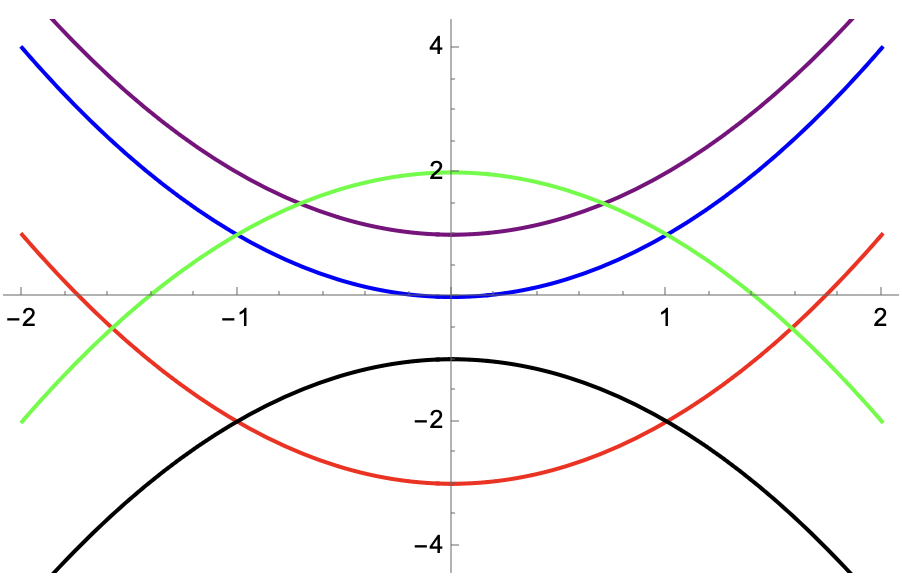
\includegraphics{chapters/assets/ineq/quadplots.png}}
		\caption{}
		\label{fig:quad}
	\end{figure*}
	\begin{enumerate}
		\item There are no solutions.
		\item There is one solution.
		\item There is a connected interval of solutions between the two zeros.
		\item There is a disjoint interval of solutions around the two zeros.
		\item Every real number satisfies the inequality.
	\end{enumerate}
	Therefore, if the quadratic has one solution, then the inequality has no solutions, if the quadratic has no solutions, then the inequality has either no solutions or every real number is a solution. If there are exactly 2 solutions, then the quadric has either a connected or disjoint interval of solutions. Let's see which scenario we have here. Solving the quadric gives
	$$x^2+3x+2=0$$
	$$(x+2)(x+1)=0$$
	hence
	$$x=\{-2,-1\}.$$
	Therefore our inequality has either a connected or disjoint interval. To figure out which one it is, we just need to test a point. I usually just use 0, but note this only works if 0 is not a zero of our polynomial. Substituting 0:
	$$(0)^2+3(0)+2=2\not\le 0$$
	Since $0$ is in the disjoint portion of or quadratic, we conclude
	$$x\in[-2,-1]$$
	satisfies our inequality.
\end{ex}

\subsection{Absolute Values}
To help us build up to our big topic at the end, we're going to examine inequalities involving absolute values.

First, we are going to examine a couple of basic properties of the absolute value. We know, by just thinking about it if
$$|x|<c$$
obviously requiring $c>0$, then
$$-c<x<c$$
The implication here goes both ways, so if
$$-c<x<c,$$
then that also implies
$$|x|<c$$

Then if we have
$$c<|x|$$
then instead of getting a connected interval, here we would get a disjoint one, with
$$x>c \jor x < -c$$
The implication here also goes both ways. Now with this, let's attempt to prove our first theorem.

\begin{theorem}[Triangle Inequality]
	Suppose $x,y\in\real$, then
	$$|x|+|y|\ge |x+y|$$
	\label{thm:triangle}
\end{theorem}
\begin{proof}
	By the definition of the absolute value,
	$$-|x|\le x \le |x|$$
	$$-|y|\le y \le |y|$$
	Therefore adding the two inequalities gives
	$$-(|x|+|y|)\le x+y \le |x|+|y|$$
	This implies
	$$|x+y|\le ||x|+|y||$$
	Since $|x|+|y|\ge 0$,
	$$|x+y|\le |x|+|y|$$
\end{proof}

\begin{cor}
	Suppose $x,y\in\real$, then
	$$||x|-|y||\le |x-y|$$
	\label{cor:invtri}
\end{cor}
\begin{proof}
	For this one, we are going to define the variable $a=x-y$. Therefore by theorem \eqref{thm:triangle},
	$$|a|+|y|\ge|a+y|=|x|$$
	Therefore
	$$|x-y|\ge |x|-|y|$$
	Then letting $b=y-x$, by. theorem \eqref{thm:triangle},
	$$|x|+|b|\ge|x+b|=|y|$$
	implying
	$$|y-x|\ge|y|-|x|$$
	$$|x-y|\ge-(|x|-|y|)$$
	$$-|x-y|\le |x|-|y|$$
	Therefore
	$$-|x-y|\le |x|-|y|\le |x-y|$$
	implying
	$$|x-y|\ge ||x|-|y||$$
\end{proof}

\section{Bounds}
\subsection{Bounded Functions}
\begin{define}
Let $f:\real\to\real$ be bounded above. Then there exists $M\in\real$ such that
for any $x\in\real$, $M\ge f(x)$.
\end{define}
\begin{define}
	Let $f:\real\to\real$ be bounded below. Then there exists $M\in\real$ such that for any $x\in\real$, $M\le f(x)$.
\end{define}
\begin{define}
	Let $f:\real\to\real$ be bounded. Then there exists $M>0$ such that for any $x\in\real$, $M\ge |f(x)|$, or equivalently, $f$ has an upper and lower bound.	
\end{define}
Now, to present these concepts more visually, we examine the function $f(x)=\frac{\sin(x)}{x}$. 
In figure \eqref{fig:upper}, we can see I've bound the function by $y=1.2,1.5,1.8$. 
\begin{figure*}[h]
	\centering
	\resizebox{0.6\textwidth}{!}{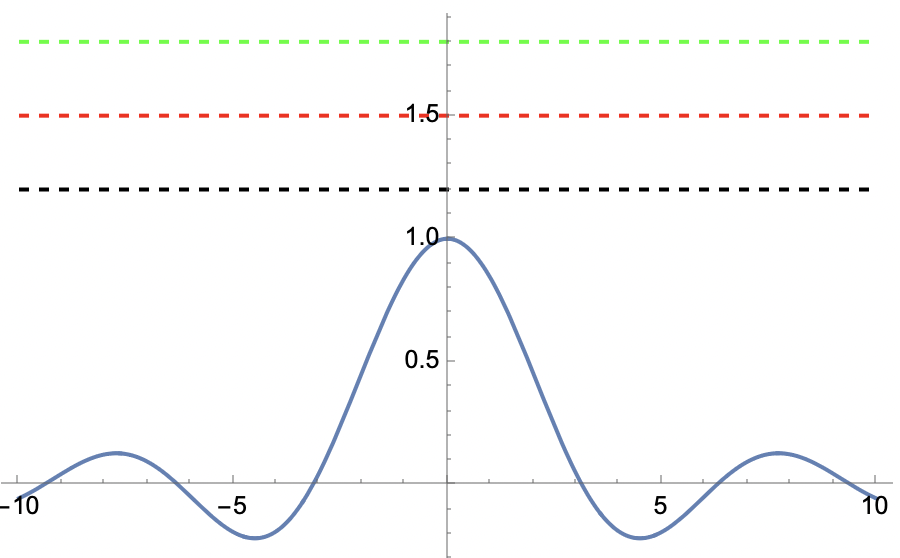
\includegraphics{chapters/assets/ineq/upperbound.png}}
	\caption{}
	\label{fig:upper}
\end{figure*}
Now since the definition of a bounded function only requires a bound to exist, not necessarily the least, we could have used any of these values for our $M$.\footnote{
It turns out that because of our existence of a finite bound, the least upper bound must exist by the Axiom of Completeness since we are working in real numbers. This is a special property of the real numbers which is not true in general. This idea helps us define what we mean by the real numbers.}

This same goes for choosing a lower bound as in figure \eqref{fig:lower}.
\begin{figure*}[h]
	\centering
	\resizebox{0.6\textwidth}{!}{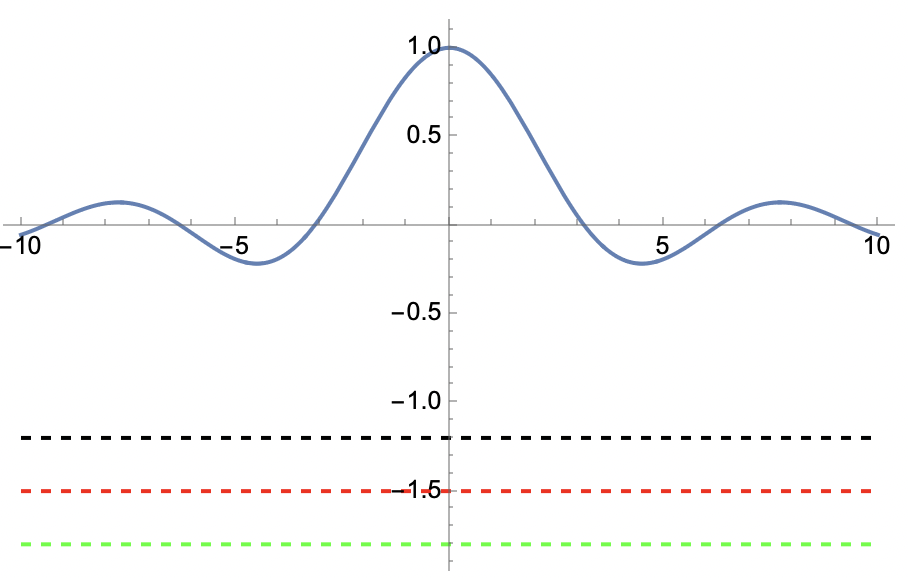
\includegraphics{chapters/assets/ineq/lowerbound.png}}
	\caption{}
	\label{fig:lower}
\end{figure*}

Now let's use this idea to prove some theorems.

\begin{theorem}
Let $f:\real\to\real$ and $g:\real\to\real$ be bounded functions. Then
\begin{enumerate}
	\item $f+g$ is bounded,
	\item $f-g$ is bounded,
	\item $f\cdot g$ is bounded.
\end{enumerate}	
\end{theorem}
\begin{proof}
	Since $f$ and $g$ are bounded, there exists $M,N>0$ such that
	$$|f(x)|\le M \jand |g(x)|\le N$$
	Then
	$$|f(x)+g(x)|\le |f(x)|+|g(x)|\le M+N$$
	which proves (1). The proof of (2) follows exactly as (1).
	
	Then since
	$$|f(x)||g(x)|=|f(x)g(x)|\le MN,$$
	This implies $f\cdot g$ is bounded, proving (3).
\end{proof}

\subsection{Limits}
Limits are a concept that will be vital for your understanding of calculus. In precalc, we are going to introduce this idea so you can become familiar with it moving into calculus.

A limit put simply is just the value a function gets closer and closer to, even if the function doesn't reach this value. The limit allows us to give meaning to discontinuities that would otherwise be undefined. In figure \eqref{fig:limit},
\begin{figure*}[h]
	\centering
	\resizebox{0.6\textwidth}{!}{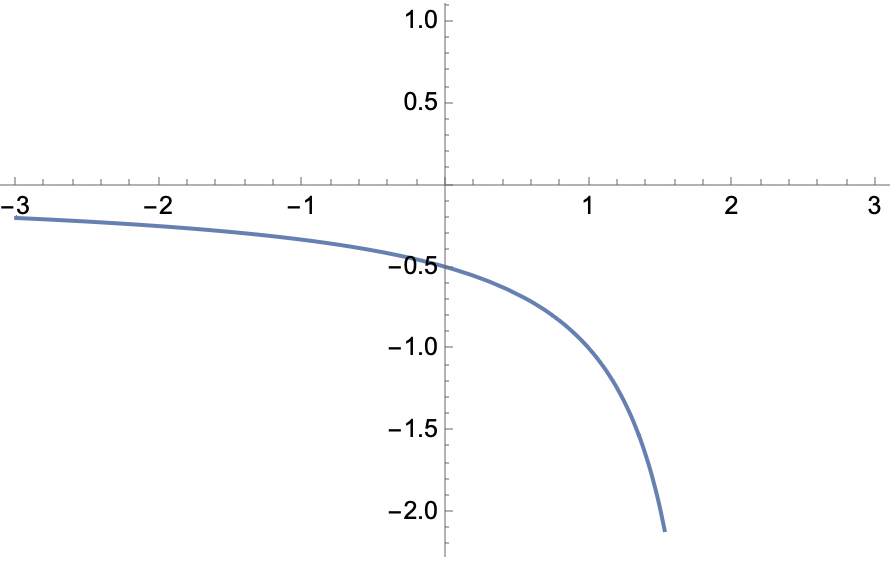
\includegraphics{chapters/assets/ineq/limitplot.png}}
	\caption{}
	\label{fig:limit}
\end{figure*}
we see the plot of $f(x)=\frac{x-1}{(x-1)(x-2)}$. By finding the maximum possible domain from this function, we get the set
$$\mathcal{D}=\{x:x\neq1,x\neq 2\}$$
For $x=2$, the function is going to infinity, so we are going to ignore that. But for $x=1$, the function clearly \textit{wants} to output a value, but just can't because of the divides by zero error.
This is where the limit comes in handy because, with the limit, we can observe the behavior around $x=1$ to assign a meaningful value to the function.

Now another way to characterize the limit is by computing values closer and closer to the problem. 
In figure \eqref{fig:computelimit}, we observe as we get closer to $x=1$, the value of the function gets closer and closer to $-1$, which is indeed what we get when we compute the limit of $f$ as $x$ approaches 1.
\begin{figure*}[h]
	\centering
	\begin{tabular}{ |c|c| }
		\hline
		$x$ & $f(x)$ \\
		\hline
		0.9 & -0.909 \\
		0.95 & -0.952\\
		0.99 & -0.990 \\
		0.999 & -0.999 \\
		\hline
		\hline
		1.001 & -1.001 \\
		1.01 & -1.010 \\
		1.05 & -1.053 \\
		1.1 & -1.111 \\
		\hline
	\end{tabular}
	\caption{}
	\label{fig:computelimit}
\end{figure*} 
Now this seems quite contrary to the rigor that we often associate with mathematics, so let's rigorously define this concept.

\begin{define}
Suppose $f:\real\to\real$\footnotemark such that
$$\lim_{x\to c}	f(x)=L,$$
where $L$ is finite, then for every $\epsilon>0$, there exists $\delta>0$ such that for all $x\neq c$, $|x-c|<\delta$ implies $|f(x)-L|<\epsilon$.
\label{def:limit}
\end{define}
\footnotetext{There is no sense in talking about limits for anything other than $\complex$ or $\real$, since a sense of connectedness must exist for this to make sense. There are other sets in which this sense of a limit exists, we call those sets topological spaces.}

That might be very hard to take and might be our hardest concept yet, but let's explain the meaning behind this using the idea of bounds.
When we write $|x-c|$, what we are computing here is just the distance between two points in the real numbers. This might seem obvious to some, but this is super important in understanding this definition.
Therefore here, the $\delta$ and $\epsilon$ can be understood as the bounds of the distance between $x$ and $c$, our point in question, and $f(x)$ and $L$ respectively.

Now the important part is that the bound on $|f(x)-L|$ can be arbitrarily small, since $\epsilon>0$, and for every $\epsilon$, we can find an interval for $x$, with radius $\delta$ around $c$ such that $|f(x)-L|$ on this interval is bounded by $\epsilon$. In other words, we can bound $|f(x)-L|$ by an arbitrarily small number by shrinking our domain around $c$.

Now let's see what we mean by if the limit doesn't exist. If the limit doesn't exist, then there exists some $\epsilon$ which cannot be a bound for $|f(x)-L|$ no matter how small we shrink the interval around $c$ for any $L$. We can see in figure \eqref{fig:nolimit} 
\begin{figure*}[h]
	\centering
	\resizebox{0.6\linewidth}{!}{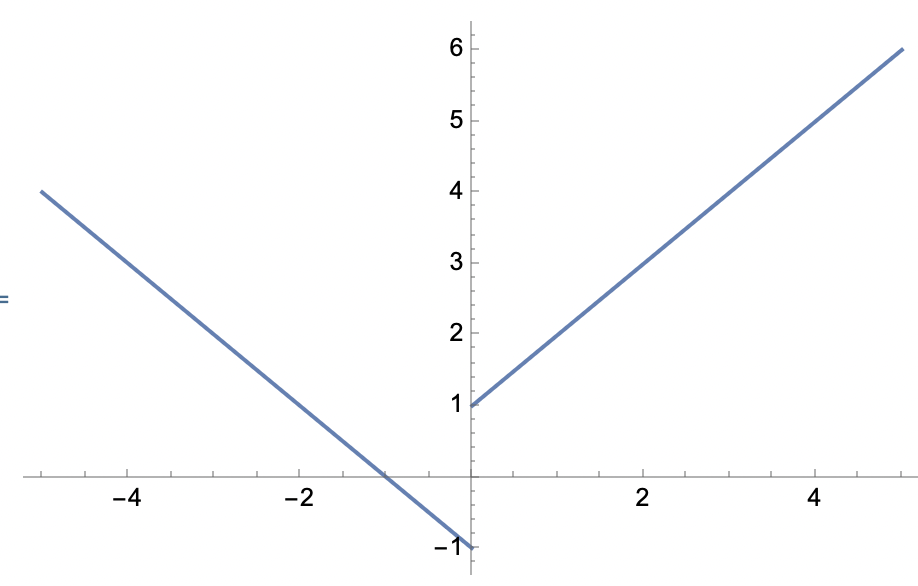
\includegraphics{chapters/assets/ineq/nolimit.png}}
	\caption{}
	\label{fig:nolimit}
\end{figure*}
that no matter how much we shrink the interval around 0, we cannot bound $|f(x)-L|$ by $\epsilon=0.5$. Therefore, we conclude the limit around 0 doesn't exist for $f(x)$.

\begin{ex}
	Let's use definition \eqref{def:limit} to prove
	$$\lim_{x\to3}\frac{x^2-9}{x-3}=6$$
	To do this, we would need a way to show that every interval around 3 exists so we can bound a $|f(x)-3|$ for any $\epsilon$. To do this, we typically try to find a function that outputs working $\delta$s for any given $\epsilon$. After we find this function, all we have to do is prove that this function works within our definition of the limit.
	
	This part because it's not part of the proof doesn't have to be as precise, so long as we can justify our findings later in a more rigorous proof. So let's try finding.
	$$\epsilon=\abs{\frac{x^2-9}{x-3}-6}.$$
	Since when talking about the limit around $3$, $x\neq3$, let's divide it out of our expression.
	$$\epsilon=\abs{x+3-6}=|x-3|$$
	Since we want a delta such that
	$$|x-3|<\delta$$
	therefore
	$$\epsilon<\delta$$
	Since we overestimated for $\epsilon$ anyway, it might be sensible to set
	$$\epsilon=\delta.$$
	Let's see if this choice works in a proof. Starting with $|x-3|<\delta$, since
	$$|x-3|=|x+3-6|=\abs{\frac{x^2-9}{x-3}-6}<\delta=\epsilon,$$
	we have shown for every $\epsilon$, we can find a delta such that the above is true, implying
	$$\lim_{x\to3}\frac{x^2-9}{x-3}=6$$
\end{ex}

\begin{ex}
	In this example, let's show
	$$\lim_{x\to2}x^2+2x=8$$
	Let's first find a suitable definition of $\epsilon$ in terms of $\delta$.
	First, let's find
	$$|x^2+2x-8|=\epsilon$$
	$$|x+4||x-2|=\epsilon$$
	Since
	$$|x-2|<\delta$$
	Now it's here that we must mention that we might need an extra condition on $\delta$.
	Since we what our expression for $\delta$ to only depend on $\epsilon$, we cannot let
	$$\delta=\frac{\epsilon}{|x+4|}$$
	A remedy here is to set $\delta<1$. This choice here is arbitrary, but sometimes a more careful choice of this bound is needed to prove more complicated limits.
	Let's examine the utility of our condition here. Since $x<3$, by $\delta<1$,
	$$|x+4||x-2|=\epsilon<7|x-2|$$
	Then it might be sensible to set
	$$\delta=\frac{\epsilon}{7}$$
	Let's see if our choice of $\delta$ works. 
	
	Without loss of generality, we can assume $\delta<1$. Then since
	$$|x-2|<\delta=\frac{\epsilon}{7}$$
	$$7|x-2|<\epsilon$$
	Since
	$$|x+4|<|x-2|+6<\delta+6<7,$$
	chaining the two inequalities together, we get
	$$|x+4||x-2|<\epsilon$$
	$$|x^2+2x-8|<\epsilon$$
	hence proving our proposition.
\end{ex}

Now let's prove some generalized properties of limits.

\begin{theorem}
Suppose
$$\lim_{x\to c}f(x)=L \jand \lim_{x\to c}g(x)=M$$
where $L$ and $M$ are finite. Then
$$\lim_{x\to c}f(x)+\lim_{x\to c}g(x)=\lim_{x\to c}\sbrak{f(x)+g(x)}$$
\end{theorem}
\begin{proof}
	Since the limits for $f$ and $g$ exist, for every $\epsilon>0$, there exists $\delta>0$ such that for every $x$ such that $0<|x-c|<\delta$\footnote{I combined the $\delta$s by taking the least required for the two functions. We can do this because $\delta$ all this does is shrink what the bound could have been for $\epsilon$.}
	$$|f(x)-L|<\frac{\epsilon}{2} \jand |g(x)-M|<\frac{\epsilon}{2}$$
	Therefore since by the theorem \eqref{thm:triangle},
	$$|f(x)+g(x)-(L+M)|<|f(x)-L|+|g(x)-M|<\frac{\epsilon}{2}+\frac{\epsilon}{2}=\epsilon$$
	hence proving our theorem.
\end{proof}

\begin{theorem}
Suppose
$$\lim_{x\to c}f(x)=L \jand \lim_{x\to c}g(x)=M$$
where $L$ and $M$ are finite. Then
$$\lim_{x\to c}f(x)\cdot\lim_{x\to c}g(x)=\lim_{x\to c}\sbrak{f(x)\cdot(x)}$$
\end{theorem}
\begin{proof}
	Since we know the limit exists for $f$ around $c$, we know there must exist an interval $\lambda>0$ such that $0<|x-c|<\lambda$ where $f$ is bounded.\footnote{
	Use the definition of the limit to show this.}
	We set let $N$ be this bound such that 
	$$|f(x)|<N.$$
	Then without loss of generality, we let $\delta<\lambda$ so by the existence of the limit for $f$ and $g$, for every $\epsilon>0$, there exists $\delta>0$ such that for every $x$ such that $0<|x-c|<\delta<\lambda$
	$$|f(x)-L|<\frac{\epsilon}{2L} \jand |g(x)-M|<\frac{\epsilon}{2N}$$
	Then we know
	$$|f(x)g(x)-LM|=|f(x)g(x)-Mf(x)+Mf(x)-LM|$$
	$$=|f(x)(g(x)-M)+M(f(x)-L|$$
	whereby theorem \eqref{thm:triangle},
	$$\ge |f(x)(g(x)-M)|+|M(f(x)-L|=|f(x)||g(x)-M)|+|M||(f(x)-L|$$
	whereby $|f(x)|<N$,
	$$<N\paren{\frac{\epsilon}{2N}}+L\paren{\frac{\epsilon}{2L}}=\epsilon$$
	hence proving the theorem.
\end{proof}

\begin{theorem}
	$$\lim_{x\to c}f(x)=L$$
where $L\neq0$ and finite. Then
$$\frac{1}{\lim_{x\to c}f(x)}=\lim_{x\to c}\sbrak{\frac{1}{f(x)}}$$
\end{theorem}
\begin{proof}
	Since the limit exists for $f$,
	$$|f(x)-L|<\frac{|L|}{2} \for 0<|x-c|<\delta_1.$$
	Since
	$$|L|=|L+f(x)-f(x)|\ge |L-f(x)|+|f(x)|$$
	$$=|f(x)-L|+|f(x)|<\frac{|L|}{2}+|f(x)|$$
	hence
	$$\frac{|L|}{2}<|f(x)|$$
	$$\frac{1}{f(x)}<\frac{2}{|L|}$$
	Since there also exists $\delta_2$ such that
	$$|f(x)-L|<\frac{|L|^2}{2} \epsilon \for 0 <|x-c|<\delta_2$$
	If we let $\delta=\min(\delta_1,\delta_2)$, for $0<|x-c|<\delta$ we have
	$$|\frac{1}{f(x)}-\frac{1}{L}|=|\frac{L-f(x)}{Lf(x)}|$$
	$$=\abs{\frac{1}{Lf(x)}}|L-f(x)|$$
	$$=\abs{\frac{1}{Lf(x)}}|f(x)-L)|<\frac{1}{|L|}\frac{2}{|L|}|g(x)-L|$$
	$$<\frac{2}{|L|^2}|g(x)-L|<\frac{2}{|L^2|}\frac{|L|^2}{2}\epsilon$$
	$$=\epsilon.$$
	Therefore
	$$\frac{1}{\lim_{x\to c}f(x)}=\lim_{x\to c}\sbrak{\frac{1}{f(x)}}$$
\end{proof}









